\subsection{Ejercicio 3}

Para realizar la tarea TaskBatch, se creó un arreglo de tamaño $total_cpu$, donde en cada posición se guarda un valor booleano que indica si en dicho momento se genera una llamada bloqueante o no. Luego se generaron cant_bloqueos números distintos de manera aleatoria dentro del rango [0, total_cpu -1]. Al hacerlo se tuvo en cuenta el hecho de que se pueden obtener números repetidos.
En este caso, si el momento creado coincide con otro momento ya generado, se vuelve a generar otro número hasta obtenerlos a todos distintos. Para cada "momento" generado, se indica en el arreglo anteriormente nombrado, el valor de verdad true (o 1).
Finalmente, se recorre el arreglo procediendo a llamar a la función que simula los bloqueos (uso_IO) en caso de que la posicion del arreglo indique true, o a la función que simula el uso del CPU (uso_CPU) en caso contrario.

Se realizó una simulación para TaskBatch con el siguente lote de tareas:

\begin{itemize}

\item TaskBatch 10 3
\item TaskBatch 5 2
\item TaskBatch 8 4

\end{itemize}

El diagrama de Gantt obtenido es el siguiente:

\begin{figure}[h]
  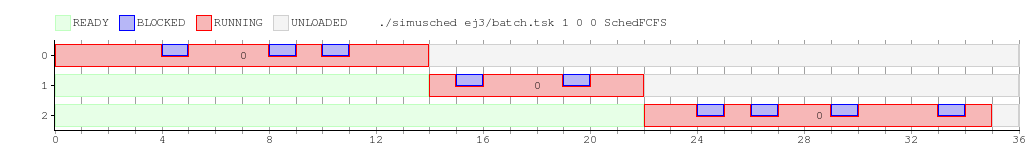
\includegraphics[width=\textwidth]{../ej3/salida.png}
  \caption{Primer lote para TaskBatch.}
  \label{fig:primera}
\end{figure}

%Cata, el ejercicio pide explicitamente 3 tareas con parametros distintos, por eso las deje. Agregue lo que me pasaste porque estaba interesante la conclusion.

En la figura ~\ref{fig:primera} se puede observar que para cada tarea, se realizan la cantidad de bloqueos pedidias. Por otra parte la duración de cada tarea equivale a la duración inicial más un cilo, con lo que concluimos que ese último ciclo correspondiente al exit() realizado por el scheduler.\\


Decidimos realizar otro lote, para verificar que la tarea funcionara adecuadamente.

\begin{itemize}

\item *3 TaskBatch 40 7

\end{itemize}

Se eligió el scheduler FCFS y un número de cores igual a la cantidad de tareas en el lote con el fin de que esté ejecutando de manera simultánea las 3 tareas y así ver efectivamente que las llamadas bloqueantes ocurren en momentos distintos para cada tarea.
El diagrama de Gantt obtenido es el siguiente:

\begin{figure}[h]
  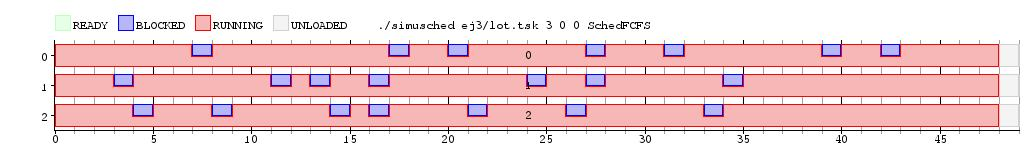
\includegraphics[width=\textwidth]{../ej3/salida2.png}
  \caption{Tareas Batch}
\end{figure}


Se puede ver fácilmente como las tres tareas hacen los llamados en momentos distintos.
